\section{Evaluating the Unfairness of Atomic Cross-Chain Swaps}
\label{sec:evaluation}

In this section, we evaluate the unfairness of Atomic Cross-Chain Swaps.

\subsection{Experimental Setting}

We collected exchange rate data of mainstream cryptocurrencies for one year, starting from May 3th 2018 to May 3th 2019.
The data was retrieved from CoinGecko.
All experiments run on a MacBook Pro with a 2.2 GHz Intel Core i7 Processor, a 16 GB DDR4 RAM and 256 SSD storage disk.

\subsection{Identifying the Unfairness by Market Volatility}

%TODO
\begin{figure}
    \includegraphics[width=\linewidth]{unfair_diagram.eps}
    \caption{Diagram showing the unfairness.}
    \label{fig:unfair_diagram}
\end{figure}

\begin{figure*}
    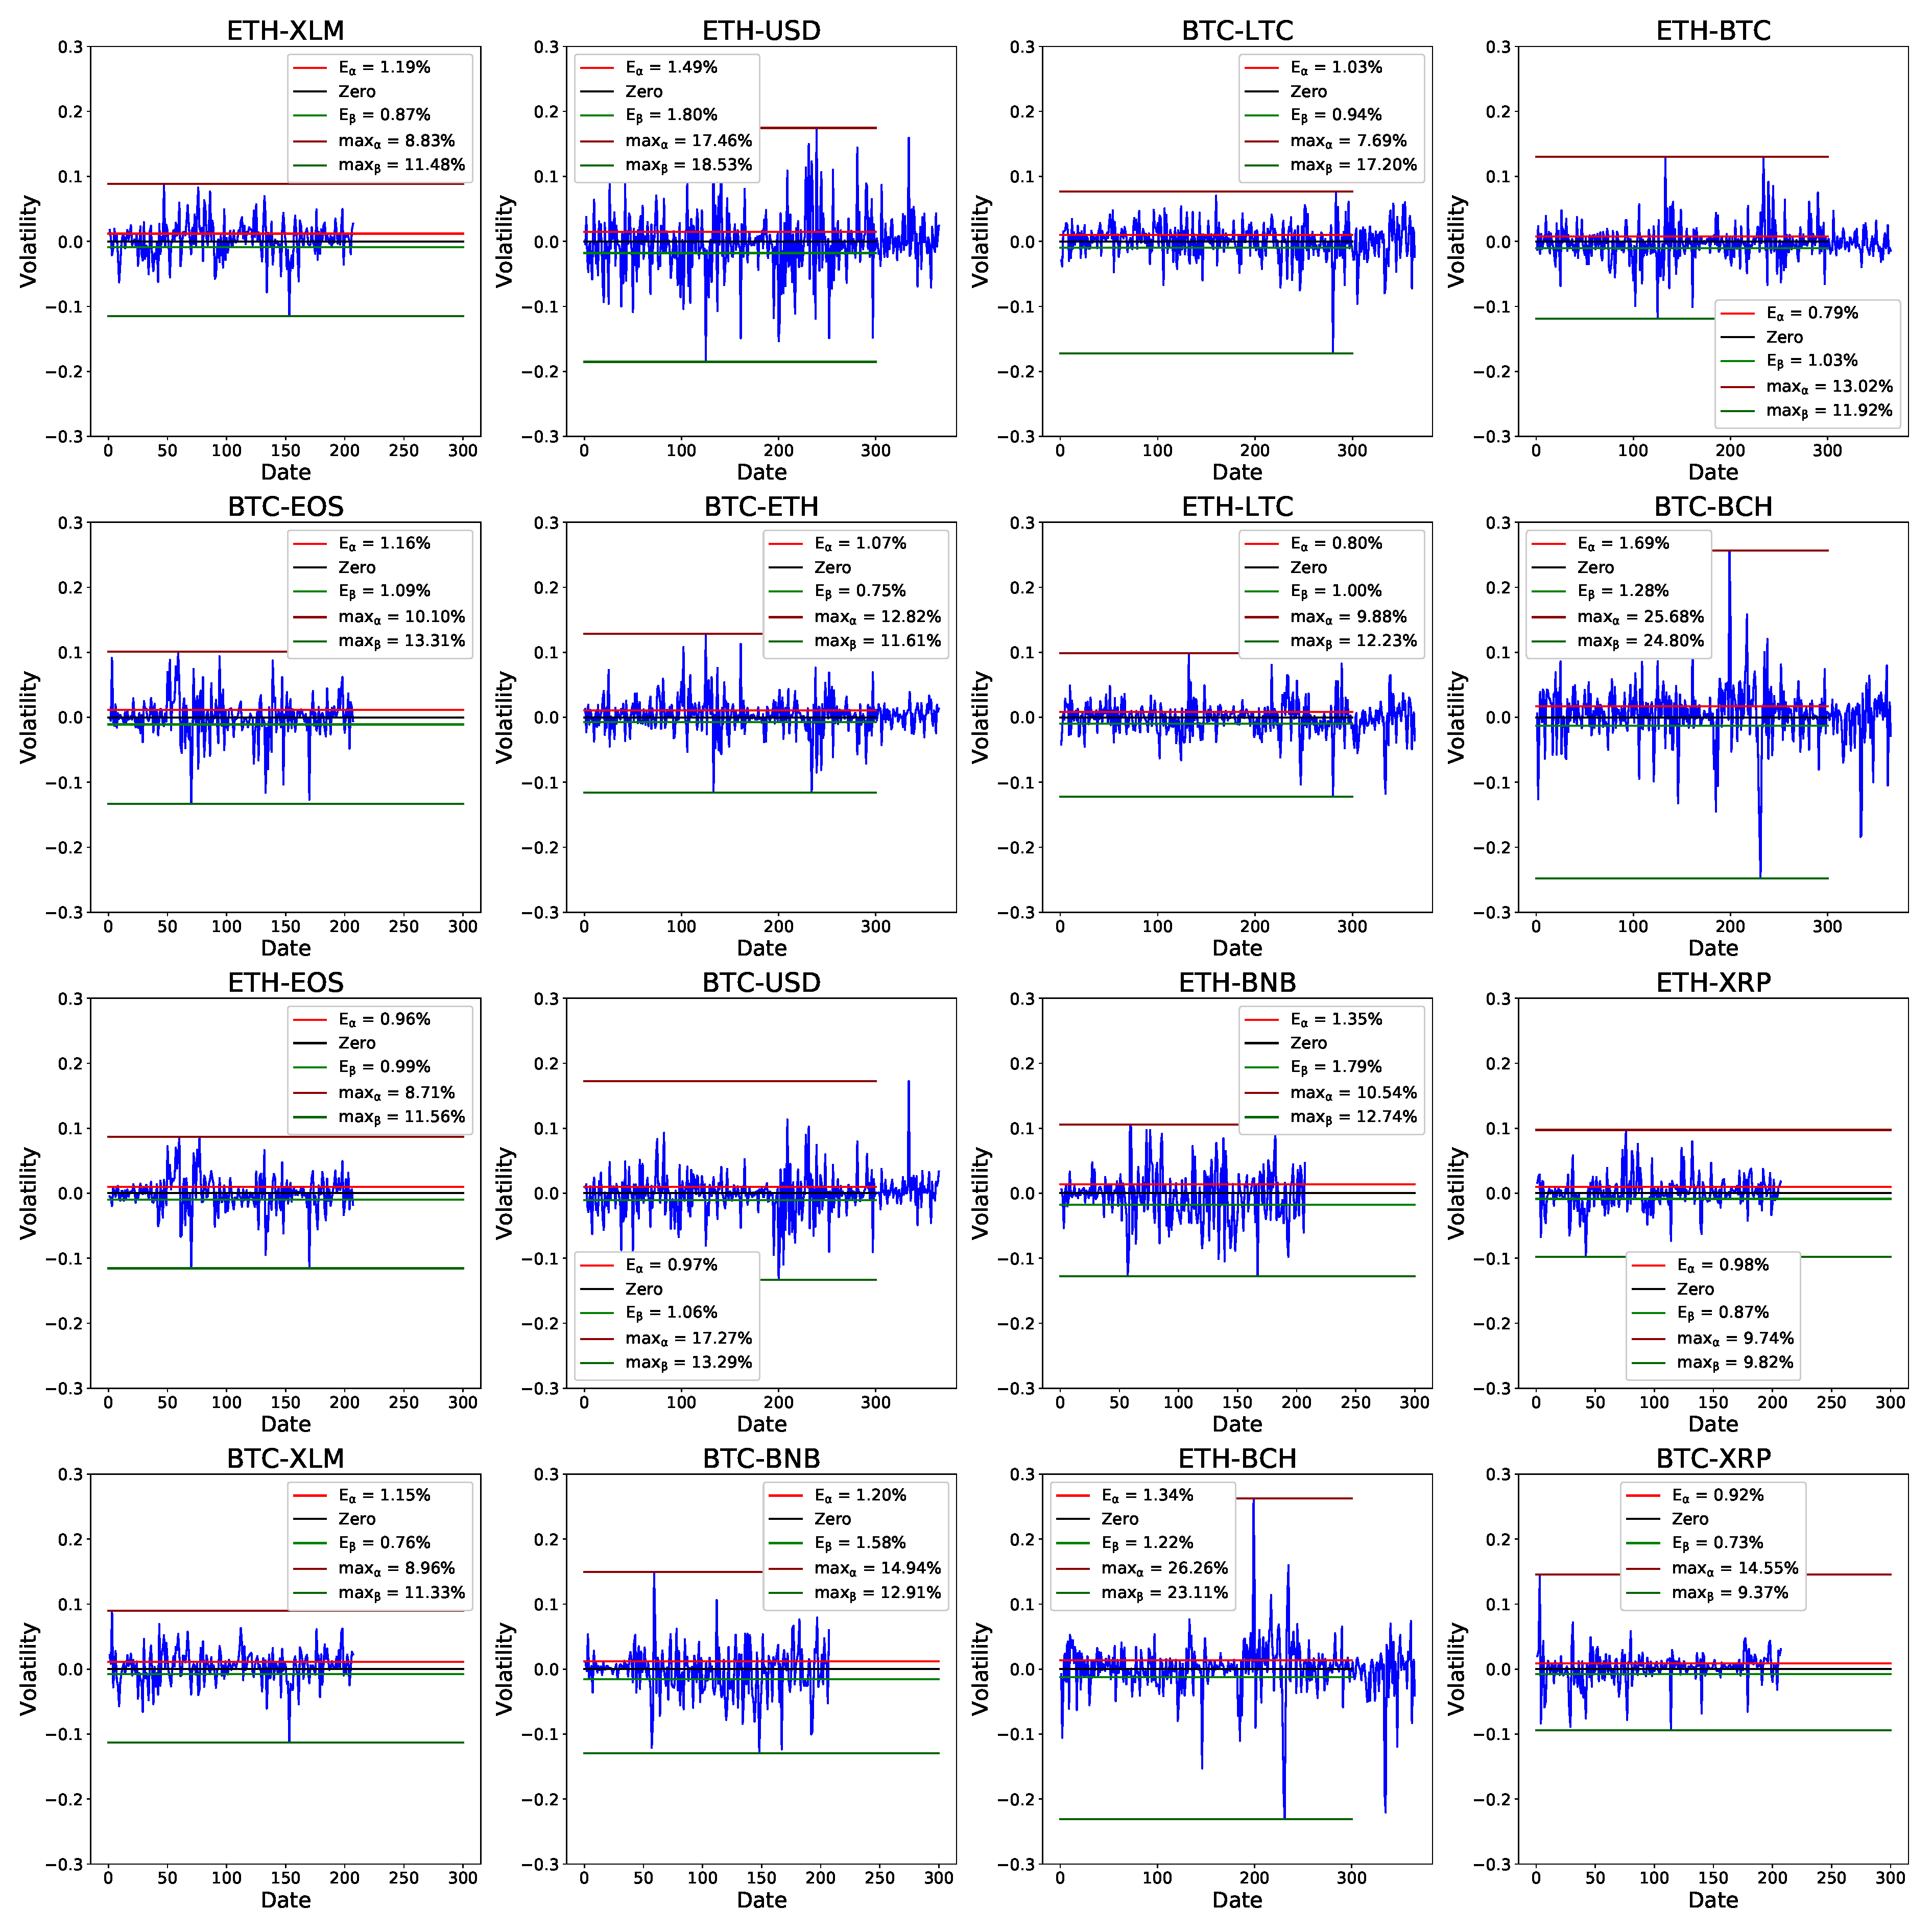
\includegraphics[width=\linewidth]{volatility_analysis.eps}
    \caption{Diagram showing the unfairness.}
    \label{fig:volatility_analysis}
\end{figure*}

\subsection{Quantifying the Unpaid Premium}

The unfair part of the Atomic Cross-Chain Swap for the participant is the unpaid premium from the initiator.
We can evaluate the unfairness of the Atomic Cross-Chain Swap by estimating the premium which should be paid by the initiator.

As the premium is the only variable in an option contract, estimating the premium is also called the ``Option Pricing'' problem.
In finance, the Black-Scholes (BS) Model is utilized to price the European Call Options,
while the Cox-Ross-Rubinstein (CRR) Model is utilized to price the American Call Options.
Therefore, we utilize the CRR Model to evaluate the unfairness of the Atomic Cross-Chain Swap.

\subsubsection{The Cox-Ross-Rubinstein Model Explained}

The CRR Model, which is also called the Binomial Options Pricing Model (BOPM), provides a generalizable numerical method for pricing the options.
Intuitively, the CRR model enumerates all possible prices of the asset in the near future based on the price volatility,
then reverse-engineers the option price based on the enumerated prices.
% binomial tree
Enumerating the possible prices utilizes a binomial tree, where each node represents a point of time.
The model assume that for each step on the binomial tree, the price rises or falls by a fixed rate.
% reverse engineering
Reverse engineering the option price relies on iteratively back propagating the option price for each level of the binomial tree.

Formally, pricing the American Call Option $\Pi = (K, \pi_1, y, \pi_2, T, pr)$ by using the CRR model is as follows:

\begin{enumerate}
    \item Creating the binomial price tree
    \item Finding the option prices for leaf nodes
    \item Finding the option prices for earlier nodes 
\end{enumerate}

\paragraph{Creating the binomial price tree}
The binomial price tree $\mathcal{T}$ of the height $n$ represents the possible future prices within the time period $T$ discretely.
$n$ can be picked arbitrarily. With larger $n$, the result will be more accurate, but the computing overhead will be heavier.
Each node $\mathcal{T}_{t, i}$ is attached with the asset price $S_{t, i}$ and the option price $C_{t, i}$,
where $t \in \{0, \frac{T}{n}, \frac{2T}{n}, \dots, T\}$ is the point of time and $i$ is the number of the node at its level.
The CRR model assumes that the asset price will either move up or down by a specific factor per step in $\mathcal{T}$.
The move-up factor is $u$, and the move-down factor is $d$.
Accordingly, the price after one move-up is $S_up = u \cdot S$, and the price after one move-down is $S_down = d \cdot S$.

$u$ and $d$ are calculated using the underlying annualized volatility $\sigma_a$ of the asset price:

\begin{align} 
u &= e^{\sigma_a \sqrt{\frac{T}{n}}}\\
d &= e^{- \sigma_a \sqrt{\frac{T}{n}}} = \frac{1}{u}
\end{align}

Here, $T$ is measured in years, and $\sigma_a$ is defined as the annual price standard deviation.
$\sigma_a$ can be computed from the daily price standard deviation $\sigma_d$ as below:

\begin{align} 
\sigma_a &= \sigma_d \sqrt{d}\\
\sigma_d &= \sqrt{\frac{\sum^{d}_{i=1} (S_i - \bar{S})^2}{d-1}}
\end{align}

where $d$ is the number of trading days within a year.
For cryptocurrencies, it equals to the number of a days within a year.

The asset price $S_{t, i}$ can also be computed as $S_{t, i} = S_{0, 1} \cdot u^{N_u - N_d}$, where $S_{0, 1}$ is the spot price, and $N_u, N_d$ are the numbers of move-up and move-down, respectively.

\paragraph{Finding the option price for each leaf node}
In the first step, only the asset prices are determined rather than the option prices.
This step further determines the option prices for leaf nodes.
For each leaf node $\mathcal{T}_{n, i}$, the option price (for Call Options) is $C_{n, i} = max[(S_{n, i} - K), 0]$.

\paragraph{Finding the option prices for earlier nodes}
We back-propagate the option prices for leaf nodes to earlier option prices.
The back propagation applies the ``risk neutrality'' assumption:
Today's fair price of a derivative equals to the expected future value discounted by the risk-free rate. % TODO further analysis
Based on this assumption, the earlier option price is calculated from the option prices of the later two nodes weighted by their state transition possibilities.
The move-up and move-down possibility are $p$ and $q$ where $p + q = 1$, and the risk-free rate is $r = q$.

The earlier option price is calculated from later option prices as:

\begin{align} 
C_{t - \Delta t, i} = e^{-r \Delta t} (p C_{t, i} + q C_{t, i+1})
\end{align}

where $p, q, r$ are computed as

\begin{align} 
p &= \frac{e^{(r-q)\Delta t} - d}{u - d}\\
q &= 1 - p\\
r &= q
\end{align}

such that the related binomial distribution simulates the geometric Brownian motion of the underlying asset value with parameters $r$ and $\sigma$.

For American Options, since the option can be exercised prior to expiry, the option price at each node is

\begin{align}
C_{t - \Delta t, i} = max[e^{-r \Delta t} (p C_{t, i} + q C_{t, i+1}), K]
\end{align}

The earliest option price $S_{0, 1}$ - the estimated option price - can be calculated by iteratively back-propagating the later option prices. 

\subsubsection{Results}

%TODO